% !TeX program = xelatex
% ============================================================
% 2002 年·全国旧课程卷·理科 · 印刷版
% 由 tools/make_editions.py 生成（重跑会覆盖本文件）；
% 题目/解析内容在 questions.tex / answers*.tex，勿在本文件内写内容。
% ============================================================
\documentclass[zihao=5, a4paper]{ctexart}
% ============================================================
% common/preamble.tex —— 拆分版试卷项目 · 公共导言区
% 引擎：XeLaTeX；文档类 ctexart 由各版本壳文件自行声明
% 由合并书 math-gaokao-2017-2026/preamble.tex 改造而来：
%   - 页眉左右改为可重定义宏 \gkheadL / \gkheadR（各版本壳设置）
%   - hyperref 不再写死 pdftitle（壳内 \hypersetup 覆盖）
%   - 删除书籍专用的 \chaptermark 重定义与 \gkpaper 装配宏
% ============================================================

% ---------- 数学 ----------
\usepackage{amsmath}
\usepackage{amssymb}
\usepackage{mathtools}

% ---------- 绘图 ----------
\usepackage{tikz}
\usetikzlibrary{shapes.geometric, arrows.meta, calc, patterns, angles, quotes, positioning}
\usepackage{pgfplots}
\pgfplotsset{compat=1.18}

% ---------- 版面 ----------
\usepackage{geometry}
\usepackage{needspace}
\geometry{a4paper, margin=2.2cm, headheight=15pt}
% 紧凑版式（如印刷版）可在壳文件中于 \begin{document} 前再次调用 \geometry 覆盖
\usepackage{enumitem}
\setlist{itemsep=2pt, topsep=4pt, parsep=0pt}

% 中文与行内公式混排的断行弹性：
% emergencystretch 允许段落末路不通时追加伸展量；
% 降低二元/关系符罚分，允许行内长公式在 = 、+ 等处断行（否则整段外溢）
\emergencystretch=2em
\binoppenalty=700
\relpenalty=500
\usepackage{booktabs}      % 三线表
\usepackage[most]{tcolorbox}

% ---------- 选择题选项对齐 ----------
% tasks 宏包：\begin{gkopts}(列数) \task ... \end{gkopts}
% 自动等宽分栏，选项天然对齐；列数已由内容片段按选项长度写定（4/2/1）
\usepackage{tasks}
\settasks{label={}, label-width=0pt, item-indent=1.2em,
          column-sep=1em, after-item-skip=2pt, before-skip=2pt, after-skip=4pt}
\NewTasksEnvironment[style=itemize]{gkopts}[\task](4)

% ---------- 页眉页脚 ----------
\newcommand{\gkheadL}{}   % 左页眉：卷名（壳文件 \renewcommand 设置）
\newcommand{\gkheadR}{}   % 右页眉：版本名（壳文件 \renewcommand 设置）
\usepackage{fancyhdr}
\pagestyle{fancy}
\fancyhf{}
\fancyhead[L]{\small\gkheadL}
\fancyhead[R]{\small\gkheadR}
\fancyfoot[C]{\small —— 第 \thepage\ 页 ——}
\renewcommand{\headrulewidth}{0.4pt}

% ---------- 超链接（须最后加载）----------
\usepackage{hyperref}
\hypersetup{colorlinks=true, linkcolor=blue!55!black,
            bookmarksnumbered=true, unicode=true}

% ============================================================
% common/macros.tex —— 自定义命令与环境（题号、解析头、提示框等）
% 与合并书 math-gaokao-2017-2026/preamble.tex 的自定义段保持一致，
% 保证内容片段（questions.tex / answers.tex）在两个项目间可互换。
% ============================================================

% ---------- 试卷标识（壳文件 \renewcommand 设置，用于 label 命名空间）----------
\newcommand{\gkpaperid}{none}

% ---------- 题号 ----------
% 试题部分的题号：加粗编号 + 自动 \label{q:<卷id>:<题号>}
\newcommand{\gkti}[1]{\par\medskip\noindent
  \textbf{#1．}\phantomsection\label{q:\gkpaperid:#1}\ignorespaces}
% 多卷/分部重启题号时，#1 是唯一内部顺序号（交叉引用身份），#2 才是原卷显示题号。
\newcommand{\gktiwithlabel}[2]{\par\medskip\noindent
  \textbf{#2．}\phantomsection\label{q:\gkpaperid:#1}\ignorespaces}

% 解析部分的题头：小标题 + 回链到试题页
% （仅在题目与解析同文档的版本中回链有效；试题版不含解析头，无悬空引用）
\newcommand{\gksolhead}[2]{%
  \Needspace{3\baselineskip}\subsubsection*{第 #1 题\if\relax\detokenize{#2}\relax\else（#2）\fi}%
  \phantomsection\label{s:\gkpaperid:#1}%
  {\small\color{gray}（题目见第~\pageref{q:\gkpaperid:#1}~页）}\par\nopagebreak}
% 与 \gktiwithlabel 成对：显示原题号，但回链仍用唯一内部顺序号。
\newcommand{\gksolheadwithlabel}[3]{%
  \Needspace{3\baselineskip}\subsubsection*{第 #2 题\if\relax\detokenize{#3}\relax\else（#3）\fi}%
  \phantomsection\label{s:\gkpaperid:#1}%
  {\small\color{gray}（题目见第~\pageref{q:\gkpaperid:#1}~页）}\par\nopagebreak}

% ---------- 填空题空位 ----------
\newcommand{\gkblank}{\underline{\hspace{2.2em}}}

% ---------- 提示框 ----------
% 卷种提示 / 解析归属声明（醒目，浅黄）
\newtcolorbox{gknotice}{colback=yellow!8, colframe=orange!60!black,
  boxrule=0.5pt, arc=1.5pt, left=6pt, right=6pt, top=4pt, bottom=4pt,
  before skip=8pt, after skip=8pt}

% 方法提示 / 注（浅蓝，用于解析后的点评与题量说明）
\newtcolorbox{gktip}{colback=blue!4, colframe=blue!35!black,
  boxrule=0.4pt, arc=1.5pt, left=6pt, right=6pt, top=4pt, bottom=4pt,
  before skip=6pt, after skip=6pt, fontupper=\small}

% ---------- 答案行 ----------
% 解析中独立成段的"答案：X"用带底色的行呈现
\newcommand{\gkanswer}[1]{\par\smallskip\noindent
  \tcbox[width=\linewidth, tcbox width=auto limited,
         colback=green!6, colframe=green!35!black, boxrule=0.4pt,
         arc=1.5pt, left=4pt, right=4pt, top=2pt, bottom=2pt,
         nobeforeafter]{\textbf{#1}}\par\smallskip}

% ---------- 结构标题 ----------
% 结构标题后通常紧跟一个带 0.5\textheight 起始预留的解析题块；0.4 只够放标题，
% 会把下一题整体推到下一页，留下孤立的「二、填空题」等页尾标题。
\newcommand{\gkpart}[1]{\Needspace{0.6\textheight}\subsection*{#1}\nopagebreak}     % 标题 + 首题
% （一）必考题 / 解析小问标题：块式加粗段，可自动换行（\paragraph 的 run-in 版式会溢出）
\newcommand{\gksubpart}[1]{\Needspace{6\baselineskip}\par\medskip\noindent\textbf{#1}\par\nopagebreak\smallskip}

% 罗马数字Ⅰ-Ⅻ（U+2160）与圈号①②③（U+2460）划入 CJK 字符类，
% 用中文字体渲染——西文字体 Latin Modern 缺这些字形，否则整段静默丢字
\xeCJKDeclareCharClass{CJK}{"2160 -> "217F, "2460 -> "24FF}

% ============================================================
% common/questions_env.tex —— 题目 / 解析的语义包装环境
%
% questions.tex 中每道题包在 \begin{question}...\end{question} 里，
% answers.tex 中每题解析包在 \begin{answer}...\end{answer} 里；
% 题头排版仍由内容行中的 \gkti / \gksolhead 完成（见 macros.tex）。
%
% 环境本身不产生任何盒子或垂直间距（只引入一个 TeX 分组），
% 排版结果与不包裹时逐点一致。它的价值在于：
%   1. 给每道题一个机器可数的结构边界（校验脚本数环境数 = 题量）；
%   2. 为将来的条件编译留钩子——某版本可重定义环境实现按题取舍。
% ============================================================

% 环境不把整题装盒：题目与解析仍可自然跨页，但开始题块前必须为题面、
% 图形/表格或解析首段留出足够空间。仅保留 2 个 baseline 会让题干、
% 选项和图形在页边界处被拆开，形成不可打印的孤立内容；题目保留
% 0.15\textheight，在避免短题制造大段空白与避免题块拆分之间取平衡。
% 解析题块保留 0.5\textheight，以容纳“题面 + 图形/选项 + 首段解析”；
% 结构标题仍用更大的保留量；末页自然收尾由视觉复审判定。
\newenvironment{question}{\Needspace{0.15\textheight}}{}
\newenvironment{answer}{\Needspace{0.5\textheight}}{}

% 紧凑版式（印刷版）：五号字由文档类选项给定；除收窄边距与压缩列表/选项间距外，
% 再压缩行距、行间公式留白与解析小标题间距。四项合计约省 11% 页数（打样卷 27 -> 24 页）。
\geometry{a4paper, margin=1.6cm, headheight=14pt}
\setlist{itemsep=1pt, topsep=2pt, parsep=0pt}
\settasks{label={}, label-width=0pt, item-indent=1.2em,
          column-sep=0.8em, after-item-skip=1pt, before-skip=1pt, after-skip=2pt}
% 行距：ctex 默认 linespread 1.3 -> 1.2（基线 16.44pt -> 15.18pt），
% 仍为字号的 1.44 倍，CJK 正文可读性不受影响。
\linespread{1.2}
% 行间公式留白：每卷解析含 150~250 个行间公式，此项是本版面最大的杠杆。
% 用 \AtBeginDocument 是因为 ctex/amsmath 会在 \begin{document} 时重置这四个长度。
\AtBeginDocument{%
  \setlength{\abovedisplayskip}{3pt plus 2pt minus 1pt}%
  \setlength{\belowdisplayskip}{3pt plus 2pt minus 1pt}%
  \setlength{\abovedisplayshortskip}{1pt plus 1pt}%
  \setlength{\belowdisplayshortskip}{2pt plus 1pt minus 1pt}}
% 标题间距：\gkpart 用 \subsection*，\gksolhead 用 \subsubsection*（每卷约 22 个）。
\ctexset{subsection/beforeskip={6pt plus 2pt minus 1pt}, subsection/afterskip={3pt plus 1pt},
         subsubsection/beforeskip={5pt plus 2pt minus 1pt}, subsubsection/afterskip={2pt plus 1pt}}
\renewcommand{\gkpaperid}{gk-2002-regular-national-old-science}
\renewcommand{\gkheadL}{2002 年·全国旧课程卷·理科 · 数学}
\renewcommand{\gkheadR}{印刷版}
\hypersetup{pdftitle={2002 年·全国旧课程卷·理科 数学 · 印刷版}}
\begin{document}
\begin{center}
  {\Large\bfseries 2002 年·全国旧课程卷·理科}\\[4pt]
  {\large 数学 · 印刷版}
\end{center}
\medskip
\pdfbookmark[1]{试题}{sec:q}
% questions.tex —— 2002 年·全国旧课程卷·理科 · 题目内容片段（无答案）
% 由 tools/generate_projects.py 依来源总账自 2002/2002_数学真题_全国旧课程理_试题.md 生成，勿手改（改源 MD 后重跑）


\gkpart{数学}

\begin{gktip}
\textbf{来源说明}：本题面依据固定源 PDF 两页 A3 题面逐题转录，原卷印刷页码 104–105。固定源不附答案，答案和解析均由本库独立复算。

\textbf{图形说明}：第 10、18 题的原卷图形关系重绘为 TikZ/PGFPlots 矢量图。图形标记所指的 PNG 不随仓库保存。
\end{gktip}

\gkpart{一、选择题}

\begin{question}
\gkti{1}圆 $(x-1)^2+y^2=1$ 的圆心到直线 $y=\dfrac{\sqrt3}{3}x$ 的距离是\mbox{（　　）}

（A）$\frac12$　　（B）$\frac{\sqrt3}{2}$　　（C）$1$　　（D）$\sqrt3$

\end{question}
\begin{question}
\gkti{2}复数

\nopagebreak[4]
\[
\left(\frac12+\frac{\sqrt3}{2}i\right)^3
\]

的值是\mbox{（　　）}

（A）$-i$　　（B）$i$　　（C）$-1$　　（D）$1$

\end{question}
\begin{question}
\gkti{3}不等式 $(1+x)(1-|x|)>0$ 的解集是\mbox{（　　）}

（A）$\{x\mid 0\leqslant x<1\}$

（B）$\{x\mid x<0\text{ \text{且} }x\neq-1\}$

（C）$\{x\mid -1<x<1\}$

（D）$\{x\mid x<1\text{ \text{且} }x\neq-1\}$

\end{question}
\begin{question}
\gkti{4}在 $(0,2\pi)$ 内，使 $\sin x>\cos x$ 成立的 $x$ 的取值范围是\mbox{（　　）}

（A）$\left(\frac\pi4,\frac\pi2\right)\cup\left(\pi,\frac{5\pi}4\right)$

（B）$\left(\frac\pi4,\pi\right)$

（C）$\left(\frac\pi4,\frac{5\pi}4\right)$

（D）$\left(\frac\pi4,\pi\right)\cup\left(\frac{5\pi}4,\frac{3\pi}2\right)$

\end{question}
\begin{question}
\gkti{5}设集合

\nopagebreak[4]
\[
M=\left\{x\middle|x=\frac{k}{2}+\frac14,\ k\in\mathbb Z\right\},\qquad
N=\left\{x\middle|x=\frac{k}{4}+\frac12,\ k\in\mathbb Z\right\},
\]

则\mbox{（　　）}

（A）$M=N$　　（B）$M\subseteq N$　　（C）$M\supseteq N$　　（D）$M\cap N=\varnothing$

\end{question}
\begin{question}
\gkti{6}点 $P(1,0)$ 到曲线

\nopagebreak[4]
\[
\begin{cases}
x=t^2,\\
y=2t,
\end{cases}
\qquad t\in\mathbb R
\]

上的点的最短距离为\mbox{（　　）}

（A）$0$　　（B）$1$　　（C）$\sqrt2$　　（D）$2$

\end{question}
\begin{question}
\gkti{7}一个圆锥和一个半球有公共底面，如果圆锥的体积恰好与半球的体积相等，那么这个圆锥轴截面顶角的余弦值是\mbox{（　　）}

（A）$\frac34$　　（B）$\frac45$　　（C）$\frac35$　　（D）$-\frac35$

\end{question}
\begin{question}
\gkti{8}正六棱柱 $ABCDEF-A_1B_1C_1D_1E_1F_1$ 的底面边长为 $1$，侧棱长为 $\sqrt2$，则这个棱柱侧面对角线 $E_1D$ 与 $BC_1$ 所成的角是\mbox{（　　）}

（A）$90^\circ$　　（B）$60^\circ$　　（C）$45^\circ$　　（D）$30^\circ$

\end{question}
\begin{question}
\gkti{9}函数 $y=x^2+bx+c$，$x\in[0,+\infty)$ 是单调函数的充要条件是\mbox{（　　）}

（A）$b\geqslant0$　　（B）$b\leqslant0$　　（C）$b>0$　　（D）$b<0$

\Needspace{0.4\textheight}
\end{question}
\begin{question}
\gkti{10}函数

\nopagebreak[4]
\[
y=1-\frac{1}{x-1}
\]

的图象是\mbox{（　　）}
\nopagebreak[4]
\begin{center}% 2002 年全国旧课程理科第 10 题：函数图象选项
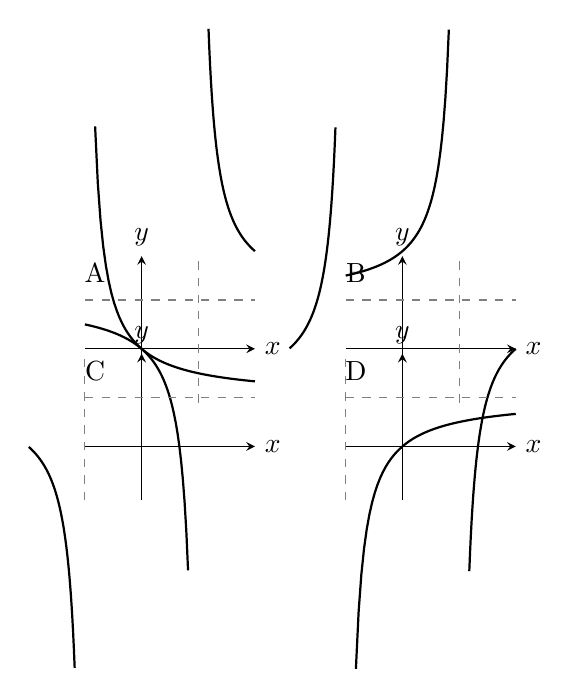
\begin{tikzpicture}[x=0.72cm,y=0.62cm,>=stealth]
  \foreach \sx/\sy/\optlabel in {0/2/A,4.6/2/B,0/0/C,4.6/0/D}
  {
    \begin{scope}[shift={(\sx,\sy)}]
      \draw[->] (-1.0,0)--(2.0,0) node[right] {$x$};
      \draw[->] (0,-1.1)--(0,1.9) node[above] {$y$};
      \node at (-0.82,1.55) {\optlabel};
    \end{scope}
  }
  % A: y=1+1/(x-1)
  \begin{scope}[shift={(0,2)}]
    \draw[dashed,gray] (1,-1.1)--(1,1.9);
    \draw[dashed,gray] (-1,1)--(2,1);
    \draw[thick,domain=-1:0.82,samples=60] plot (\x,{1+1/(\x-1)});
    \draw[thick,domain=1.18:2,samples=60] plot (\x,{1+1/(\x-1)});
  \end{scope}
  % B: y=1-1/(x-1), the correct graph
  \begin{scope}[shift={(4.6,2)}]
    \draw[dashed,gray] (1,-1.1)--(1,1.9);
    \draw[dashed,gray] (-1,1)--(2,1);
    \draw[thick,domain=-1:0.82,samples=60] plot (\x,{1-1/(\x-1)});
    \draw[thick,domain=1.18:2,samples=60] plot (\x,{1-1/(\x-1)});
  \end{scope}
  % C and D use x=-1, distinguishing the remaining distractors.
  \begin{scope}[shift={(0,0)}]
    \draw[dashed,gray] (-1,-1.1)--(-1,1.9);
    \draw[dashed,gray] (-1,1)--(2,1);
    \draw[thick,domain=-0.82:2,samples=60] plot (\x,{1+1/(\x+1)});
    \draw[thick,domain=-1.99:-1.18,samples=60] plot (\x,{1+1/(\x+1)});
  \end{scope}
  \begin{scope}[shift={(4.6,0)}]
    \draw[dashed,gray] (-1,-1.1)--(-1,1.9);
    \draw[dashed,gray] (-1,1)--(2,1);
    \draw[thick,domain=-0.82:2,samples=60] plot (\x,{1-1/(\x+1)});
    \draw[thick,domain=-1.99:-1.18,samples=60] plot (\x,{1-1/(\x+1)});
  \end{scope}
\end{tikzpicture}
\end{center}
\nopagebreak[4]
（A）　　（B）　　（C）　　（D）

\end{question}
\begin{question}
\gkti{11}从正方体的 6 个面中选取 3 个面，其中有 2 个面不相邻的选法共有\mbox{（　　）}

（A）8 种　　（B）12 种　　（C）16 种　　（D）20 种

\end{question}
\begin{question}
\gkti{12}据 2002 年 3 月 5 日九届人大五次会议《政府工作报告》：“2001 年国内生产总值达到 95933 亿元，比上年增长 $7.3\%\mbox{\fontspec{STSong}\char"3002}$”如果“十五”（2001—2005 年）期间每年的国内生产总值都按此年增长率增长，那么到“十五”末我国国内年生产总值约为\mbox{（　　）}

（A）115000 亿元　　（B）120000 亿元　　（C）127000 亿元　　（D）135000 亿元

\end{question}
\gkpart{二、填空题}

\begin{question}
\gkti{13}函数 $y=a^x$ 在 $[0,1]$ 上的最大值与最小值之和为 $3$，则 $a=$\gkblank{}。

\end{question}
\begin{question}
\gkti{14}椭圆 $5x^2+ky^2=5$ 的一个焦点是 $(0,2)$，那么 $k=$\gkblank{}。

\end{question}
\begin{question}
\gkti{15}$(x^2+1)(x-2)^7$ 展开式中 $x^3$ 的系数是\gkblank{}。

\end{question}
\begin{question}
\gkti{16}已知

\nopagebreak[4]
\[
f(x)=\frac{x^2}{1+x^2},
\]

\Needspace{5\baselineskip}
那么

\nopagebreak[4]
\[
f(1)+f(2)+f\left(\frac12\right)+f(3)+f\left(\frac13\right)+f(4)+f\left(\frac14\right)=\_\_\_\_\_\_\mbox{\fontspec{STSong}\char"3002}
\]

\end{question}
\gkpart{三、解答题}

\begin{question}
\gkti{17}已知

\nopagebreak[4]
\[
\sin^2 2\alpha+\sin2\alpha\cos\alpha-\cos2\alpha=1,\qquad
\alpha\in\left(0,\frac\pi2\right),
\]

求 $\sin\alpha\text{、}\tan\alpha$ 的值。

\Needspace{0.4\textheight}
\end{question}
\begin{question}
\gkti{18}如图，正方形 $ABCD\text{、}ABEF$ 的边长都是 $1$，而且平面 $ABCD\text{、}ABEF$ 互相垂直。点 $M$ 在 $AC$ 上移动，点 $N$ 在 $BF$ 上移动，若 $CM=BN=a$（$0<a<\sqrt2$）。
\nopagebreak[4]
\begin{center}% 2002 年全国旧课程理科第 18 题：两个互相垂直的正方形
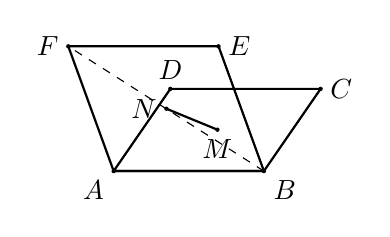
\begin{tikzpicture}[>=stealth,scale=0.72]
  \coordinate (A) at (0,0);
  \coordinate (B) at (2.65,0);
  \coordinate (C) at (3.65,1.45);
  \coordinate (D) at (1.0,1.45);
  \coordinate (E) at (1.85,2.20);
  \coordinate (F) at (-0.80,2.20);
  \coordinate (M) at (1.83,0.73);
  \coordinate (N) at (0.93,1.10);
  \draw[thick] (A)--(B)--(C)--(D)--cycle;
  \draw[thick] (A)--(B)--(E)--(F)--cycle;
  \draw[dashed] (A)--(D) (B)--(F);
  \draw[thick] (M)--(N);
  \fill (A) circle (1.1pt) node[below left] {$A$};
  \fill (B) circle (1.1pt) node[below right] {$B$};
  \fill (C) circle (1.1pt) node[right] {$C$};
  \fill (D) circle (1.1pt) node[above] {$D$};
  \fill (E) circle (1.1pt) node[right] {$E$};
  \fill (F) circle (1.1pt) node[left] {$F$};
  \fill (M) circle (1.1pt) node[below] {$M$};
  \fill (N) circle (1.1pt) node[left] {$N$};
\end{tikzpicture}
\end{center}
\nopagebreak[4]
（1） 求 $MN$ 的长；

（2） $a$ 为何值时，$MN$ 的长最小；

（3） 当 $MN$ 的长最小时，求面 $MNA$ 与面 $MNB$ 所成二面角 $\alpha$ 的大小。

\end{question}
\begin{question}
\gkti{19}设点 $P$ 到点 $(-1,0)\text{、}(1,0)$ 距离之差为 $2m$，到 $x\text{、}y$ 轴的距离之比为 $2$，求 $m$ 的取值范围。

\end{question}
\begin{question}
\gkti{20}某城市 2001 年末汽车保有量为 30 万辆，预计此后每年报废上一年末汽车保有量的 $6\%$，并且每年新增汽车数量相同。为保护城市环境，要求该城市汽车保有量不超过 60 万辆，那么每年新增汽车数量不应超过多少辆？

\end{question}
\begin{question}
\gkti{21}设 $a$ 为实数，函数

\nopagebreak[4]
\[
f(x)=x^2+|x-a|+1,\qquad x\in\mathbb R.
\]

（1） 讨论 $f(x)$ 的奇偶性；

（2） 求 $f(x)$ 的最小值。

\end{question}
\begin{question}
\gkti{22}设数列 $\{a_n\}$ 满足

\nopagebreak[4]
\[
a_{n+1}=a_n^2-na_n+1,\qquad n=1,2,3,\ldots.
\]

（1） 当 $a_1=2$ 时，求 $a_2,a_3,a_4$，并由此猜测 $a_n$ 的一个通项公式；

（2） 当 $a_1\geqslant3$ 时，证明对所有的 $n\geqslant1$，有

① $a_n\geqslant n+2$；

\Needspace{5\baselineskip}
②

\nopagebreak[4]
\[
\frac1{1+a_1}+\frac1{1+a_2}+\frac1{1+a_3}+\cdots+\frac1{1+a_n}\leqslant\frac12.
\]

\end{question}
\par\bigskip\hrule\bigskip
\pdfbookmark[1]{参考答案与详细解析}{sec:s}
\Needspace{8\baselineskip}
\begin{center}{\large\bfseries 参考答案与详细解析}\end{center}
\smallskip
% answers.tex —— 2002 年·全国旧课程卷·理科 · 参考答案与详细解析片段
% 由 tools/generate_projects.py 依来源总账自 2002/2002_数学真题_全国旧课程理_试题.md + 2002/2002_数学真题_全国旧课程理_解析正文.md + 2002/2002_数学真题_全国旧课程理_答案要点.md 生成，勿手改（改源 MD 后重跑）


\begin{gktip}
固定源 PDF 为印刷页码 104–105 的两页题面，不附答案。以下解析均依据题面独立复算；第 10、18 题图形在 LaTeX 工程中以 TikZ/PGFPlots 矢量源重绘。
\end{gktip}

\gkpart{一、选择题}

\begin{answer}
\gksolhead{1}{}

\textbf{题目}：

圆 $(x-1)^2+y^2=1$ 的圆心到直线 $y=\dfrac{\sqrt3}{3}x$ 的距离是\mbox{（　　）}

（A）$\frac12$　　（B）$\frac{\sqrt3}{2}$　　（C）$1$　　（D）$\sqrt3$

\Needspace{4\baselineskip}
\textbf{解析}

\Needspace{5\baselineskip}
直线写成

\nopagebreak[4]
\[
\sqrt3x-3y=0.
\]

\Needspace{5\baselineskip}
圆心为 $(1,0)$，故圆心到直线的距离为

\nopagebreak[4]
\[
\frac{\sqrt3}{\sqrt{(\sqrt3)^2+(-3)^2}}
=\frac12.
\]

故选 A。

\gkanswer{答案：A}

\end{answer}
\begin{answer}
\gksolhead{2}{}

\textbf{题目}：

\Needspace{5\baselineskip}
复数

\nopagebreak[4]
\[
\left(\frac12+\frac{\sqrt3}{2}i\right)^3
\]

的值是\mbox{（　　）}

（A）$-i$　　（B）$i$　　（C）$-1$　　（D）$1$

\Needspace{4\baselineskip}
\textbf{解析}

\Needspace{5\baselineskip}
同样由棣莫弗定理，

\nopagebreak[4]
\[
\left(\frac12+\frac{\sqrt3}{2}i\right)^3
=\cos\pi+i\sin\pi=-1.
\]

故选 C。

\gkanswer{答案：C}

\end{answer}
\begin{answer}
\gksolhead{3}{}

\textbf{题目}：

不等式 $(1+x)(1-|x|)>0$ 的解集是\mbox{（　　）}

（A）$\{x\mid 0\leqslant x<1\}$

（B）$\{x\mid x<0\text{ \text{且} }x\neq-1\}$

（C）$\{x\mid -1<x<1\}$

（D）$\{x\mid x<1\text{ \text{且} }x\neq-1\}$

\Needspace{4\baselineskip}
\textbf{解析}

\Needspace{5\baselineskip}
分 $x\geqslant0$ 和 $x<0$ 讨论，分别得到 $0\leqslant x<1$ 以及 $x<0$ 且 $x\neq-1$。合并为

\nopagebreak[4]
\[
x<1,\qquad x\neq-1.
\]

故选 D。

\gkanswer{答案：D}

\end{answer}
\begin{answer}
\gksolhead{4}{}

\textbf{题目}：

在 $(0,2\pi)$ 内，使 $\sin x>\cos x$ 成立的 $x$ 的取值范围是\mbox{（　　）}

（A）$\left(\frac\pi4,\frac\pi2\right)\cup\left(\pi,\frac{5\pi}4\right)$

（B）$\left(\frac\pi4,\pi\right)$

（C）$\left(\frac\pi4,\frac{5\pi}4\right)$

（D）$\left(\frac\pi4,\pi\right)\cup\left(\frac{5\pi}4,\frac{3\pi}2\right)$

\Needspace{4\baselineskip}
\textbf{解析}

\Needspace{5\baselineskip}
在 $(0,2\pi)$ 内，

\nopagebreak[4]
\[
\sin x>\cos x
\Longleftrightarrow
\sin\left(x-\frac\pi4\right)>0,
\]

\Needspace{5\baselineskip}
所以

\nopagebreak[4]
\[
x\in\left(\frac\pi4,\frac{5\pi}4\right).
\]

故选 C。

\gkanswer{答案：C}

\end{answer}
\begin{answer}
\gksolhead{5}{}

\textbf{题目}：

\Needspace{5\baselineskip}
设集合

\nopagebreak[4]
\[
M=\left\{x\middle|x=\frac{k}{2}+\frac14,\ k\in\mathbb Z\right\},\qquad
N=\left\{x\middle|x=\frac{k}{4}+\frac12,\ k\in\mathbb Z\right\},
\]

则\mbox{（　　）}

（A）$M=N$　　（B）$M\subseteq N$　　（C）$M\supseteq N$　　（D）$M\cap N=\varnothing$

\Needspace{4\baselineskip}
\textbf{解析}

\Needspace{5\baselineskip}
有

\nopagebreak[4]
\[
M=\left\{\frac{2k+1}{4}\middle|k\in\mathbb Z\right\}
\subseteq
\left\{\frac{j}{4}\middle|j\in\mathbb Z\right\}=N.
\]

故选 B。

\gkanswer{答案：B}

\end{answer}
\begin{answer}
\gksolhead{6}{}

\textbf{题目}：

\Needspace{5\baselineskip}
点 $P(1,0)$ 到曲线

\nopagebreak[4]
\[
\begin{cases}
x=t^2,\\
y=2t,
\end{cases}
\qquad t\in\mathbb R
\]

上的点的最短距离为\mbox{（　　）}

（A）$0$　　（B）$1$　　（C）$\sqrt2$　　（D）$2$

\Needspace{4\baselineskip}
\textbf{解析}

\Needspace{5\baselineskip}
曲线上点为 $(t^2,2t)$，所以点 $P(1,0)$ 到该点的距离平方为

\nopagebreak[4]
\[
d^2=(t^2-1)^2+(2t)^2
=t^4+2t^2+1
=(t^2+1)^2.
\]

当 $t=0$ 时取最小值 $1$，故最短距离为 $1$，选 B。

\gkanswer{答案：B}

\end{answer}
\begin{answer}
\gksolhead{7}{}

\textbf{题目}：

一个圆锥和一个半球有公共底面，如果圆锥的体积恰好与半球的体积相等，那么这个圆锥轴截面顶角的余弦值是\mbox{（　　）}

（A）$\frac34$　　（B）$\frac45$　　（C）$\frac35$　　（D）$-\frac35$

\Needspace{4\baselineskip}
\textbf{解析}

\Needspace{5\baselineskip}
设圆锥底面半径为 $r$、高为 $h$。由体积相等得 $h=2r$。轴截面顶角的余弦为

\nopagebreak[4]
\[
\frac{h^2-r^2}{h^2+r^2}
=\frac35.
\]

故选 C。

\gkanswer{答案：C}

\end{answer}
\begin{answer}
\gksolhead{8}{}

\textbf{题目}：

正六棱柱 $ABCDEF-A_1B_1C_1D_1E_1F_1$ 的底面边长为 $1$，侧棱长为 $\sqrt2$，则这个棱柱侧面对角线 $E_1D$ 与 $BC_1$ 所成的角是\mbox{（　　）}

（A）$90^\circ$　　（B）$60^\circ$　　（C）$45^\circ$　　（D）$30^\circ$

\Needspace{4\baselineskip}
\textbf{解析}

\Needspace{5\baselineskip}
在正六边形底面中取边长为 $1$ 的坐标表示

\nopagebreak[4]
\[
A=(1,0),\quad
B=\left(\frac12,\frac{\sqrt3}{2}\right),\quad
C=\left(-\frac12,\frac{\sqrt3}{2}\right),\quad
D=(-1,0),\quad
E=\left(-\frac12,-\frac{\sqrt3}{2}\right).
\]

\Needspace{5\baselineskip}
令侧棱方向为 $z$ 轴，则

\nopagebreak[4]
\[
\overrightarrow{DE_1}
=\left(\frac12,-\frac{\sqrt3}{2},\sqrt2\right),
\qquad
\overrightarrow{BC_1}=(-1,0,\sqrt2).
\]

\Needspace{5\baselineskip}
两向量的长度均为 $\sqrt3$，内积为

\nopagebreak[4]
\[
\overrightarrow{DE_1}\cdot\overrightarrow{BC_1}
=-\frac12+2=\frac32.
\]

\Needspace{5\baselineskip}
因此直线所成的角 $\theta$ 满足

\nopagebreak[4]
\[
\cos\theta=\frac{3/2}{3}=\frac12,
\qquad\theta=60^\circ.
\]

故选 B。

\gkanswer{答案：B}

\end{answer}
\begin{answer}
\gksolhead{9}{}

\textbf{题目}：

函数 $y=x^2+bx+c$，$x\in[0,+\infty)$ 是单调函数的充要条件是\mbox{（　　）}

（A）$b\geqslant0$　　（B）$b\leqslant0$　　（C）$b>0$　　（D）$b<0$

\Needspace{4\baselineskip}
\textbf{解析}

\nopagebreak[4]
\[
y'=2x+b.
\]

在 $[0,+\infty)$ 上成为单调函数的充要条件是 $2x+b\geqslant0$ 对所有 $x\geqslant0$ 成立，即 $b\geqslant0$。故选 A。

\gkanswer{答案：A}

\end{answer}
\begin{answer}
\gksolhead{10}{}

\textbf{题目}：

\Needspace{5\baselineskip}
函数

\nopagebreak[4]
\[
y=1-\frac{1}{x-1}
\]

的图象是\mbox{（　　）}
\nopagebreak[4]
\begin{center}% 2002 年全国旧课程理科第 10 题：函数图象选项
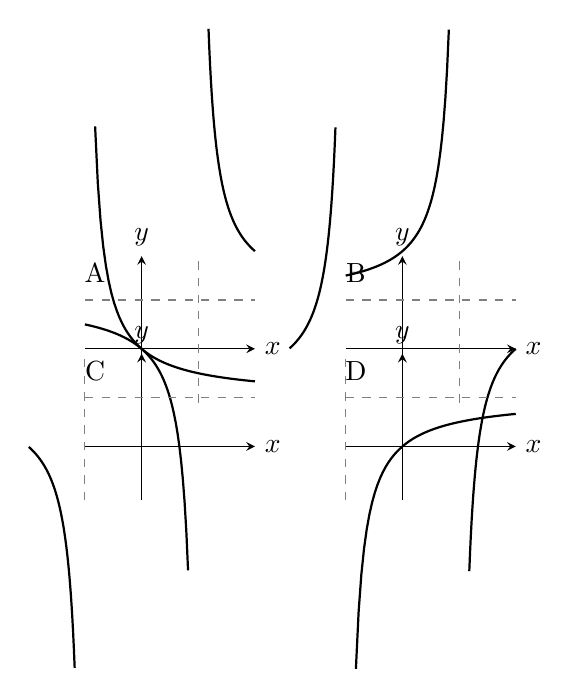
\begin{tikzpicture}[x=0.72cm,y=0.62cm,>=stealth]
  \foreach \sx/\sy/\optlabel in {0/2/A,4.6/2/B,0/0/C,4.6/0/D}
  {
    \begin{scope}[shift={(\sx,\sy)}]
      \draw[->] (-1.0,0)--(2.0,0) node[right] {$x$};
      \draw[->] (0,-1.1)--(0,1.9) node[above] {$y$};
      \node at (-0.82,1.55) {\optlabel};
    \end{scope}
  }
  % A: y=1+1/(x-1)
  \begin{scope}[shift={(0,2)}]
    \draw[dashed,gray] (1,-1.1)--(1,1.9);
    \draw[dashed,gray] (-1,1)--(2,1);
    \draw[thick,domain=-1:0.82,samples=60] plot (\x,{1+1/(\x-1)});
    \draw[thick,domain=1.18:2,samples=60] plot (\x,{1+1/(\x-1)});
  \end{scope}
  % B: y=1-1/(x-1), the correct graph
  \begin{scope}[shift={(4.6,2)}]
    \draw[dashed,gray] (1,-1.1)--(1,1.9);
    \draw[dashed,gray] (-1,1)--(2,1);
    \draw[thick,domain=-1:0.82,samples=60] plot (\x,{1-1/(\x-1)});
    \draw[thick,domain=1.18:2,samples=60] plot (\x,{1-1/(\x-1)});
  \end{scope}
  % C and D use x=-1, distinguishing the remaining distractors.
  \begin{scope}[shift={(0,0)}]
    \draw[dashed,gray] (-1,-1.1)--(-1,1.9);
    \draw[dashed,gray] (-1,1)--(2,1);
    \draw[thick,domain=-0.82:2,samples=60] plot (\x,{1+1/(\x+1)});
    \draw[thick,domain=-1.99:-1.18,samples=60] plot (\x,{1+1/(\x+1)});
  \end{scope}
  \begin{scope}[shift={(4.6,0)}]
    \draw[dashed,gray] (-1,-1.1)--(-1,1.9);
    \draw[dashed,gray] (-1,1)--(2,1);
    \draw[thick,domain=-0.82:2,samples=60] plot (\x,{1-1/(\x+1)});
    \draw[thick,domain=-1.99:-1.18,samples=60] plot (\x,{1-1/(\x+1)});
  \end{scope}
\end{tikzpicture}
\end{center}
\nopagebreak[4]
（A）　　（B）　　（C）　　（D）

\Needspace{4\baselineskip}
\textbf{解析}

\Needspace{5\baselineskip}
函数

\nopagebreak[4]
\[
y=1-\frac1{x-1}
\]

的竖直渐近线为 $x=1$，水平渐近线为 $y=1$。当 $x<1$ 时，$x-1<0$，所以 $y>1$；当 $x>1$ 时，$y<1$。因此图象位于渐近线左上和右下两个区域，对应选项 B。

\gkanswer{答案：B}

\end{answer}
\begin{answer}
\gksolhead{11}{}

\textbf{题目}：

从正方体的 6 个面中选取 3 个面，其中有 2 个面不相邻的选法共有\mbox{（　　）}

（A）8 种　　（B）12 种　　（C）16 种　　（D）20 种

\Needspace{4\baselineskip}
\textbf{解析}

\Needspace{5\baselineskip}
从三组相对面中选一组，再从其余四个面中选第三个面，共

\nopagebreak[4]
\[
3\times4=12
\]

种，故选 B。

\gkanswer{答案：B}

\end{answer}
\begin{answer}
\gksolhead{12}{}

\textbf{题目}：

据 2002 年 3 月 5 日九届人大五次会议《政府工作报告》：“2001 年国内生产总值达到 95933 亿元，比上年增长 $7.3\%\mbox{\fontspec{STSong}\char"3002}$”如果“十五”（2001—2005 年）期间每年的国内生产总值都按此年增长率增长，那么到“十五”末我国国内年生产总值约为\mbox{（　　）}

（A）115000 亿元　　（B）120000 亿元　　（C）127000 亿元　　（D）135000 亿元

\Needspace{4\baselineskip}
\textbf{解析}

\Needspace{5\baselineskip}
到“十五”末经过四个年度增长，国内生产总值约为

\nopagebreak[4]
\[
95933(1.073)^4\approx127000
\]

亿元，故选 C。

\gkanswer{答案：C}

\end{answer}
\gkpart{二、填空题}

\begin{answer}
\gksolhead{13}{}

\textbf{题目}：

函数 $y=a^x$ 在 $[0,1]$ 上的最大值与最小值之和为 $3$，则 $a=$\gkblank{}。

\Needspace{4\baselineskip}
\textbf{解析}

若 $a>1$，最大值与最小值分别为 $a\text{、}1$，由 $a+1=3$ 得 $a=2$；若 $0<a<1$，和小于 $2$。故 $a=2$。

\gkanswer{答案：$2$}

\end{answer}
\begin{answer}
\gksolhead{14}{}

\textbf{题目}：

椭圆 $5x^2+ky^2=5$ 的一个焦点是 $(0,2)$，那么 $k=$\gkblank{}。

\Needspace{4\baselineskip}
\textbf{解析}

\Needspace{5\baselineskip}
椭圆方程化为

\nopagebreak[4]
\[
x^2+\frac{k}{5}y^2=1.
\]

\Needspace{5\baselineskip}
焦点 $(0,2)$ 给出

\nopagebreak[4]
\[
\frac5k-1=4,
\]

所以 $k=1$。

\gkanswer{答案：$1$}

\end{answer}
\begin{answer}
\gksolhead{15}{}

\textbf{题目}：

$(x^2+1)(x-2)^7$ 展开式中 $x^3$ 的系数是\gkblank{}。

\Needspace{4\baselineskip}
\textbf{解析}

\nopagebreak[4]
\[
[x^3]\bigl((x^2+1)(x-2)^7\bigr)
=\binom71(-2)^6+\binom73(-2)^4
=448+560=1008.
\]

\gkanswer{答案：$1008$}

\end{answer}
\begin{answer}
\gksolhead{16}{}

\textbf{题目}：

\Needspace{5\baselineskip}
已知

\nopagebreak[4]
\[
f(x)=\frac{x^2}{1+x^2},
\]

\Needspace{5\baselineskip}
那么

\nopagebreak[4]
\[
f(1)+f(2)+f\left(\frac12\right)+f(3)+f\left(\frac13\right)+f(4)+f\left(\frac14\right)=\_\_\_\_\_\_\mbox{\fontspec{STSong}\char"3002}
\]

\Needspace{4\baselineskip}
\textbf{解析}

\Needspace{5\baselineskip}
对任意 $x\neq0$，

\nopagebreak[4]
\[
f(x)+f\left(\frac1x\right)
=\frac{x^2}{1+x^2}+\frac{1}{1+x^2}=1.
\]

\Needspace{5\baselineskip}
因此

\nopagebreak[4]
\[
f(2)+f\left(\frac12\right)
=f(3)+f\left(\frac13\right)
=f(4)+f\left(\frac14\right)=1,
\]

\Needspace{5\baselineskip}
而 $f(1)=1/2$，总和为

\nopagebreak[4]
\[
\frac12+1+1+1=\frac72.
\]

\gkanswer{答案：$\dfrac72$}

\end{answer}
\gkpart{三、解答题}

\begin{answer}
\gksolhead{17}{}

\textbf{题目}：

\Needspace{5\baselineskip}
已知

\nopagebreak[4]
\[
\sin^2 2\alpha+\sin2\alpha\cos\alpha-\cos2\alpha=1,\qquad
\alpha\in\left(0,\frac\pi2\right),
\]

求 $\sin\alpha\text{、}\tan\alpha$ 的值。

\Needspace{4\baselineskip}
\textbf{解析}

\Needspace{5\baselineskip}
令 $s=\sin\alpha$、$c=\cos\alpha$。因 $\alpha\in(0,\pi/2)$，有 $s,c>0$。原式化为

\nopagebreak[4]
\[
4s^2c^2+2sc^2-(c^2-s^2)=1.
\]

\Needspace{5\baselineskip}
利用 $s^2+c^2=1$ 整理得

\nopagebreak[4]
\[
2c^2(2s^2+s-1)=0.
\]

\Needspace{5\baselineskip}
由于 $c\neq0$，故

\nopagebreak[4]
\[
2s^2+s-1=0.
\]

\Needspace{5\baselineskip}
取正根得 $s=1/2$，从而 $c=\sqrt3/2$，所以

\nopagebreak[4]
\[
\sin\alpha=\frac12,\qquad
\tan\alpha=\frac{\sqrt3}{3}.
\]

\gkanswer{答案：$\sin\alpha=\dfrac12$，$\tan\alpha=\dfrac{\sqrt3}{3}$。}

\end{answer}
\begin{answer}
\gksolhead{18}{}

\textbf{题目}：

如图，正方形 $ABCD\text{、}ABEF$ 的边长都是 $1$，而且平面 $ABCD\text{、}ABEF$ 互相垂直。点 $M$ 在 $AC$ 上移动，点 $N$ 在 $BF$ 上移动，若 $CM=BN=a$（$0<a<\sqrt2$）。
\nopagebreak[4]
\begin{center}% 2002 年全国旧课程理科第 18 题：两个互相垂直的正方形
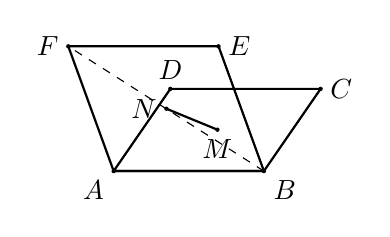
\begin{tikzpicture}[>=stealth,scale=0.72]
  \coordinate (A) at (0,0);
  \coordinate (B) at (2.65,0);
  \coordinate (C) at (3.65,1.45);
  \coordinate (D) at (1.0,1.45);
  \coordinate (E) at (1.85,2.20);
  \coordinate (F) at (-0.80,2.20);
  \coordinate (M) at (1.83,0.73);
  \coordinate (N) at (0.93,1.10);
  \draw[thick] (A)--(B)--(C)--(D)--cycle;
  \draw[thick] (A)--(B)--(E)--(F)--cycle;
  \draw[dashed] (A)--(D) (B)--(F);
  \draw[thick] (M)--(N);
  \fill (A) circle (1.1pt) node[below left] {$A$};
  \fill (B) circle (1.1pt) node[below right] {$B$};
  \fill (C) circle (1.1pt) node[right] {$C$};
  \fill (D) circle (1.1pt) node[above] {$D$};
  \fill (E) circle (1.1pt) node[right] {$E$};
  \fill (F) circle (1.1pt) node[left] {$F$};
  \fill (M) circle (1.1pt) node[below] {$M$};
  \fill (N) circle (1.1pt) node[left] {$N$};
\end{tikzpicture}
\end{center}
\nopagebreak[4]
（1） 求 $MN$ 的长；

（2） $a$ 为何值时，$MN$ 的长最小；

（3） 当 $MN$ 的长最小时，求面 $MNA$ 与面 $MNB$ 所成二面角 $\alpha$ 的大小。

\Needspace{4\baselineskip}
\textbf{解析}

\Needspace{5\baselineskip}
取

\nopagebreak[4]
\[
A=(0,0,0),\quad B=(1,0,0),\quad C=(1,1,0),\quad D=(0,1,0),
\]

\Needspace{5\baselineskip}
并令正方形 $ABEF$ 位于 $xz$ 平面，取 $E=(1,0,1)$、$F=(0,0,1)$。设

\nopagebreak[4]
\[
r=\frac{a}{\sqrt2}.
\]

\Needspace{5\baselineskip}
由于 $CM=BN=a$，可写为

\nopagebreak[4]
\[
M=(1-r,1-r,0),\qquad
N=(1-r,0,r).
\]

\gksubpart{(1)}

\Needspace{5\baselineskip}
于是

\nopagebreak[4]
\[
MN^2=(1-r)^2+r^2
=1-\sqrt2a+a^2,
\]

\Needspace{5\baselineskip}
所以

\nopagebreak[4]
\[
MN=\sqrt{a^2-\sqrt2a+1}.
\]

\gksubpart{(2)}

\Needspace{5\baselineskip}
配方得

\nopagebreak[4]
\[
MN^2=\left(a-\frac{\sqrt2}{2}\right)^2+\frac12.
\]

\Needspace{5\baselineskip}
故当

\nopagebreak[4]
\[
a=\frac{\sqrt2}{2}
\]

时 $MN$ 最小。

\gksubpart{(3)}

\Needspace{5\baselineskip}
此时

\nopagebreak[4]
\[
M=\left(\frac12,\frac12,0\right),\qquad
N=\left(\frac12,0,\frac12\right).
\]

\Needspace{5\baselineskip}
设 $H$ 为 $MN$ 的中点，则 $AH$、$BH$ 都垂直于 $MN$，$\angle AHB$ 是所求二面角的平面角。计算得

\nopagebreak[4]
\[
\overrightarrow{HA}
=\left(-\frac12,-\frac14,-\frac14\right),\qquad
\overrightarrow{HB}
=\left(\frac12,-\frac14,-\frac14\right).
\]

\Needspace{5\baselineskip}
两向量内积为 $-1/8$，长度平方均为 $3/8$，所以

\nopagebreak[4]
\[
\cos\alpha
=\frac{-1/8}{3/8}
=-\frac13.
\]

\Needspace{5\baselineskip}
因此

\nopagebreak[4]
\[
\alpha=\arccos\left(-\frac13\right).
\]

\gkanswer{答案（1）：$MN=\sqrt{a^2-\sqrt2a+1}$。}

\gkanswer{答案（2）：$a=\dfrac{\sqrt2}{2}$。}

\gkanswer{答案（3）：$\alpha=\arccos\left(-\dfrac13\right)$。}

\end{answer}
\begin{answer}
\gksolhead{19}{}

\textbf{题目}：

设点 $P$ 到点 $(-1,0)\text{、}(1,0)$ 距离之差为 $2m$，到 $x\text{、}y$ 轴的距离之比为 $2$，求 $m$ 的取值范围。

\Needspace{4\baselineskip}
\textbf{解析}

\Needspace{5\baselineskip}
设 $P=(x,y)$，并按题面顺序令距离之差的有向量值满足 $PM-PN=2m$；取绝对值时结论给出相应的 $|m|$ 范围。由到 $x$ 轴、$y$ 轴的距离之比为 $2$，有

\nopagebreak[4]
\[
\frac{|y|}{|x|}=2,\qquad y=\pm2x,\qquad x\neq0.
\]

\Needspace{5\baselineskip}
取 $y=2x$（另一条直线给出相同的距离范围），则

\nopagebreak[4]
\[
PM=\sqrt{5x^2+2x+1},\qquad
PN=\sqrt{5x^2-2x+1}.
\]

\Needspace{5\baselineskip}
令

\nopagebreak[4]
\[
2|m|=|PM-PN|.
\]

\Needspace{5\baselineskip}
当 $x\to0$ 时，右端趋于 $0$；当 $|x|\to+\infty$ 时，

\nopagebreak[4]
\[
|PM-PN|
\longrightarrow\frac{2}{\sqrt5}.
\]

\Needspace{5\baselineskip}
并且该差值随 $|x|$ 连续严格增加，故

\nopagebreak[4]
\[
0<2|m|<\frac{2}{\sqrt5},
\qquad\text{\text{即}}\qquad
0<|m|<\frac1{\sqrt5}.
\]

若将“距离之差”中的 $m$ 约定为非负参数，则写成 $0<m<1/\sqrt5$。

\gkanswer{答案：$0<|m|<\dfrac1{\sqrt5}$；若按“距离之差”将 $m$ 约定为非负数，则为 $0<m<\dfrac1{\sqrt5}$。}

\end{answer}
\begin{answer}
\gksolhead{20}{}

\textbf{题目}：

某城市 2001 年末汽车保有量为 30 万辆，预计此后每年报废上一年末汽车保有量的 $6\%$，并且每年新增汽车数量相同。为保护城市环境，要求该城市汽车保有量不超过 60 万辆，那么每年新增汽车数量不应超过多少辆？

\Needspace{4\baselineskip}
\textbf{解析}

\Needspace{5\baselineskip}
设每年新增汽车 $x$ 万辆，记第 $n$ 年末汽车保有量为 $a_n$，则

\nopagebreak[4]
\[
a_1=30,\qquad
a_{n+1}=0.94a_n+x.
\]

\Needspace{5\baselineskip}
若要使保有量始终不超过 $60$，新增量不能超过使稳定水平达到 $60$ 的值。稳定水平满足

\nopagebreak[4]
\[
L=0.94L+x.
\]

\Needspace{5\baselineskip}
令 $L=60$，得

\nopagebreak[4]
\[
x=(1-0.94)\times60=3.6.
\]

\Needspace{5\baselineskip}
当 $x=3.6$ 时，数列从 $30$ 单调增加并趋近于 $60$，不会超过 $60$；因此每年新增量不超过

\nopagebreak[4]
\[
3.6\text{ \text{万辆}}=36000\text{ \text{辆}}.
\]

\gkanswer{答案：不超过 $36000$ 辆。}

\end{answer}
\begin{answer}
\gksolhead{21}{}

\textbf{题目}：

\Needspace{5\baselineskip}
设 $a$ 为实数，函数

\nopagebreak[4]
\[
f(x)=x^2+|x-a|+1,\qquad x\in\mathbb R.
\]

（1） 讨论 $f(x)$ 的奇偶性；

（2） 求 $f(x)$ 的最小值。

\Needspace{4\baselineskip}
\textbf{解析}

\gksubpart{(1)}

\Needspace{5\baselineskip}
有

\nopagebreak[4]
\[
f(-x)=x^2+|-x-a|+1=x^2+|x+a|+1.
\]

要使 $f(-x)=f(x)$ 对所有 $x$ 成立，必须且只需 $a=0$。当 $a=0$ 时，$f(x)=x^2+|x|+1$，确为偶函数。

另一方面 $f(0)=|a|+1>0$，所以无论 $a$ 取何值，$f$ 都不可能是奇函数。

因此：$a=0$ 时为偶函数；任何 $a$ 下都不是奇函数。

\gksubpart{(2)}

\Needspace{5\baselineskip}
当 $x<a$ 时，

\nopagebreak[4]
\[
f(x)=x^2-x+a+1;
\]

\Needspace{5\baselineskip}
当 $x\geqslant a$ 时，

\nopagebreak[4]
\[
f(x)=x^2+x-a+1.
\]

\Needspace{5\baselineskip}
若 $-\frac12\leqslant a\leqslant\frac12$，两段的顶点均不能落在各自的内部，最小值在折点 $x=a$ 处取得：

\nopagebreak[4]
\[
f(a)=a^2+1.
\]

\Needspace{5\baselineskip}
若 $a\geqslant\frac12$，左段顶点 $x=1/2$ 可取，最小值为

\nopagebreak[4]
\[
f\left(\frac12\right)=a+\frac34.
\]

\Needspace{5\baselineskip}
若 $a\leqslant-\frac12$，右段顶点 $x=-1/2$ 可取，最小值为

\nopagebreak[4]
\[
f\left(-\frac12\right)=\frac34-a.
\]

\Needspace{5\baselineskip}
合并得

\nopagebreak[4]
\[
\min f(x)=
\begin{cases}
a^2+1,& |a|\leqslant\dfrac12,\\[4pt]
|a|+\dfrac34,& |a|\geqslant\dfrac12.
\end{cases}
\]

\gkanswer{答案（1）：当 $a=0$ 时为偶函数；不存在奇函数的情形。}

\gkanswer{答案（2）：$\min f(x)=a^2+1$（$|a|\leqslant\dfrac12$），$\min f(x)=|a|+\dfrac34$（$|a|\geqslant\dfrac12$）。}

\end{answer}
\begin{answer}
\gksolhead{22}{}

\textbf{题目}：

\Needspace{5\baselineskip}
设数列 $\{a_n\}$ 满足

\nopagebreak[4]
\[
a_{n+1}=a_n^2-na_n+1,\qquad n=1,2,3,\ldots.
\]

（1） 当 $a_1=2$ 时，求 $a_2,a_3,a_4$，并由此猜测 $a_n$ 的一个通项公式；

（2） 当 $a_1\geqslant3$ 时，证明对所有的 $n\geqslant1$，有

① $a_n\geqslant n+2$；

\Needspace{5\baselineskip}
②

\nopagebreak[4]
\[
\frac1{1+a_1}+\frac1{1+a_2}+\frac1{1+a_3}+\cdots+\frac1{1+a_n}\leqslant\frac12.
\]

\Needspace{4\baselineskip}
\textbf{解析}

\gksubpart{(1)}

\Needspace{5\baselineskip}
当 $a_1=2$ 时，

\nopagebreak[4]
\[
a_2=2^2-1\cdot2+1=3,
\]

\nopagebreak[4]
\[
a_3=3^2-2\cdot3+1=4,
\]

\nopagebreak[4]
\[
a_4=4^2-3\cdot4+1=5.
\]

\Needspace{5\baselineskip}
由此猜测 $a_n=n+1$。代回递推式验证：

\nopagebreak[4]
\[
(n+1)^2-n(n+1)+1=n+2,
\]

所以该通项确实满足递推关系及初值。

\gksubpart{(2)}

\Needspace{5\baselineskip}
先证①。由 $a_1\geqslant3$，有 $a_1\geqslant1+2$。若 $a_n\geqslant n+2$，则

\nopagebreak[4]
\[
a_{n+1}=a_n(a_n-n)+1
\geqslant a_n\cdot2+1
\geqslant2n+5
>n+3.
\]

\Needspace{5\baselineskip}
归纳得

\nopagebreak[4]
\[
a_n\geqslant n+2,\qquad n\geqslant1.
\]

\Needspace{5\baselineskip}
令

\nopagebreak[4]
\[
b_n=a_n-n-1.
\]

\Needspace{5\baselineskip}
由①知 $b_n\geqslant1$，并且

\nopagebreak[4]
\[
\begin{aligned}
b_{n+1}
&=a_{n+1}-n-2\\
&=a_n^2-na_n-n-1\\
&=b_n(b_n+n+2).
\end{aligned}
\]

\Needspace{5\baselineskip}
又

\nopagebreak[4]
\[
\frac1{1+a_n}
=\frac1{b_n+n+2}
=\frac{b_n}{b_{n+1}}.
\]

\Needspace{5\baselineskip}
由 $b_1\geqslant1$，有 $b_1+3\geqslant4$；且

\nopagebreak[4]
\[
b_2=b_1(b_1+3)\geqslant4.
\]

\Needspace{5\baselineskip}
因此可归纳得到

\nopagebreak[4]
\[
b_n+n+2\geqslant2^{n+1},\qquad n\geqslant1.
\]

\Needspace{5\baselineskip}
于是

\nopagebreak[4]
\[
\frac1{1+a_n}\leqslant\frac1{2^{n+1}}.
\]

\Needspace{5\baselineskip}
从而

\nopagebreak[4]
\[
\sum_{k=1}^n\frac1{1+a_k}
\leqslant\sum_{k=1}^{\infty}\frac1{2^{k+1}}
=\frac12.
\]

这就证明了②。

\gkanswer{答案（1）：$a_2=3,\ a_3=4,\ a_4=5$；猜测 $a_n=n+1$。}

\gkanswer{答案（2）：见解析版。}

\end{answer}
\end{document}
